%%%%%%%%%%%%%%%%%%%%%%%%%%%%%%%%%%%%%%%%%%%%%%%%%%%%%%%%%%%%%%%
%
% Welcome to Overleaf --- just edit your LaTeX on the left,
% and we'll compile it for you on the right. If you give
% someone the link to this page, they can edit at the same
% time. See the help menu above for more info. Enjoy!
%
%%%%%%%%%%%%%%%%%%%%%%%%%%%%%%%%%%%%%%%%%%%%%%%%%%%%%%%%%%%%%%%
\documentclass[border=10pt]{standalone}
%%%<
\usepackage{verbatim}

%%%>
\usepackage{pgfplots}
\pgfplotsset{width=7cm,compat=1.8}
\begin{comment}
:Title: Scatter plot with cubes
:Tags: 3D;Scatter plots;Manual
:Author: Christian Feuersänger
:Slug: scatter-cube-plot

This scatter plot example uses mark=cube* and z buffer=sort to place boxes
at each input coordinate. The color for each box is determined by point
meta={x+y+3}. The remaining keys are just for pretty printing.

The code is from the PGFPlots 1.10 manual: "4.6.4 Scatter Plots",
"Stacked Bar Plots and Nodes Near Coords".
\end{comment}
\begin{document}
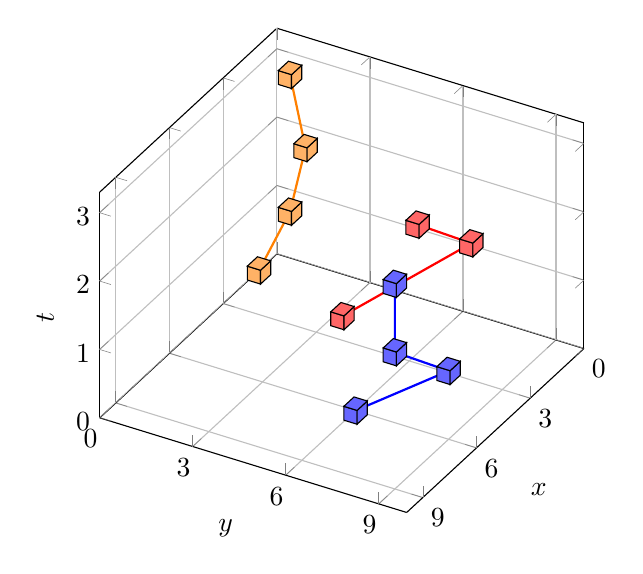
\begin{tikzpicture}
\begin{axis}[
        view={120}{40},
        width=220pt,
        height=220pt,
        grid=major,
        z buffer=sort,
        xmin=0,xmax=9,
        ymin=0,ymax=9,
        zmin=0,zmax=3,
        enlargelimits=upper,
        xtick={0,3,...,9},
        ytick={0,3,...,9},
        ztick={0,1,...,3},
        xlabel={$x$},
        ylabel={$y$},
        zlabel={$t$},
	]
    \addplot3[only marks,mark=cube*,mark size=5, fill=orange!60]
        coordinates{(1,0,0)(1,1,1)(1,1.5,2)(1,1,3)};
    \addplot3[only marks,mark=cube*,mark size=5, fill=red!60]
        coordinates{(5,5,1)(3,8,2)(6,8,3)};
    \addplot3[only marks,mark=cube*,mark size=5, fill=blue!60]
        coordinates{(6,6,0)(6,9,1)(9,9,2)(9,9,3)};
    \addplot3[thick, color=blue]   coordinates{(6,6,0)(6,9,1)(9,9,2)(9,9,3)};
    \addplot3[thick, color=red] coordinates{(6,8,3)(3,8,2)(5,5,1)};
    \addplot3[thick, color=orange] coordinates{(1,0,0)(1,1,1)(1,1.5,2)(1,1,3)};
    
\end{axis}
\end{tikzpicture}
\end{document}
